
% -------------------------------------------------------
% INSERT
% -------------------------------------------------------

\subsubsection{I2: Bulk import ocen}
\begin{figure}[H]
    \centering
    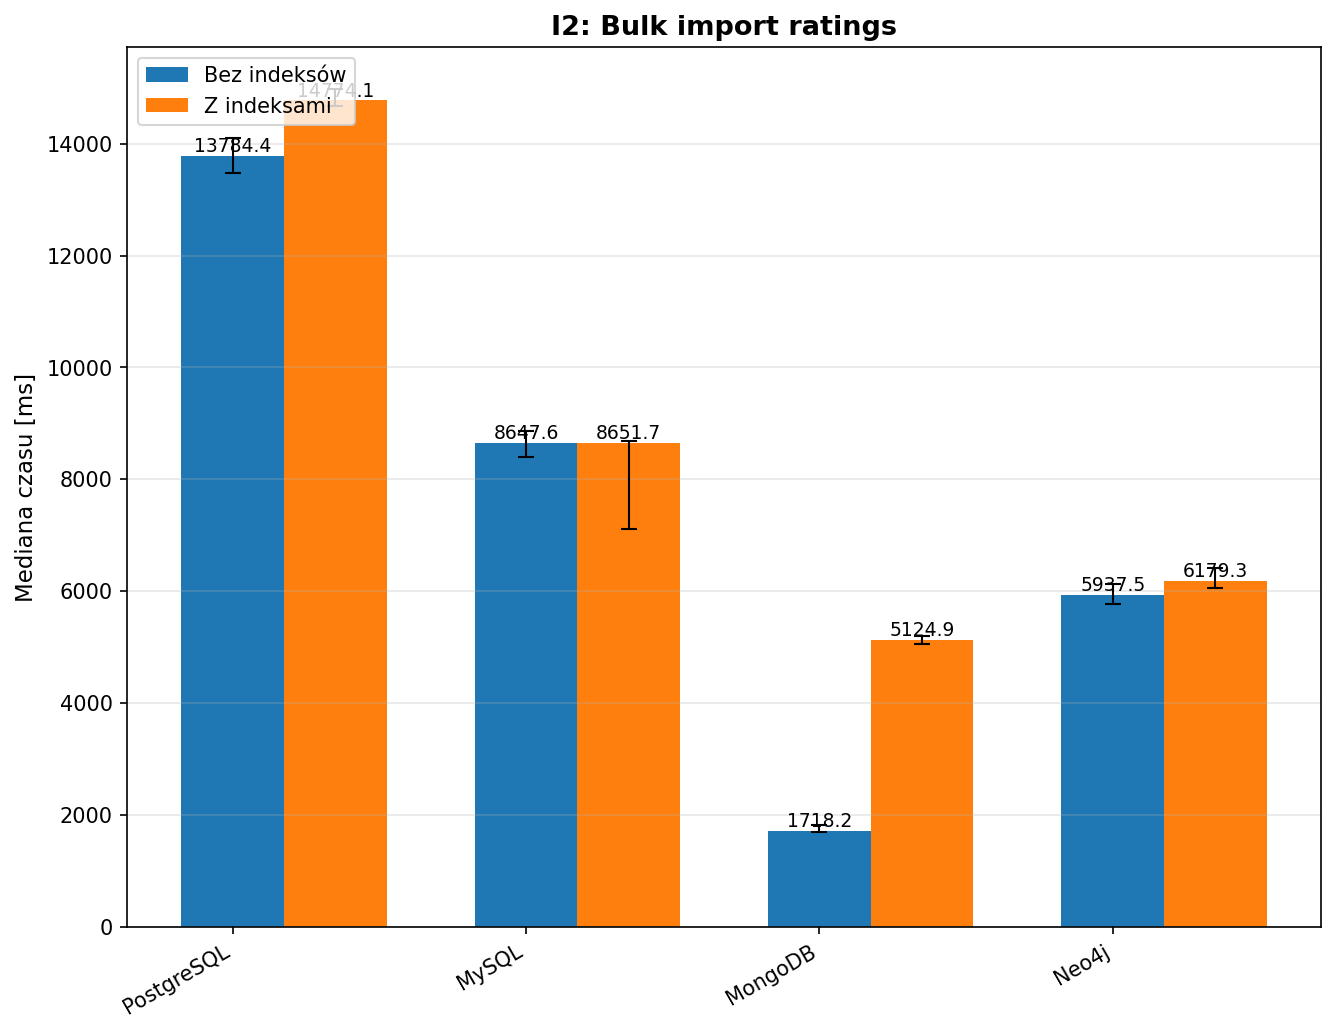
\includegraphics[width=0.8\textwidth]{charts/large/chart_I2.png}
    \caption{I2 -- Bulk import ocen}
\end{figure}

Pełna skala uwidacznia różnice między silnikami w \texttt{INSERT}-ach
masowych. PostgreSQL osiąga \emph{14~sekund} -- to konsekwencja
zarówno utrzymania WAL, jak i indeksów. MySQL 8.6~s, Neo4j 5.9~s
(co ciekawe: na małych wolumenach Neo4j był najwolniejszy, ale tu
jego architektura wsadowego \texttt{UNWIND CREATE} amortyzuje się
lepiej). MongoDB nadal najszybszy bez indeksów (1.7~s), ale z indeksami
zwalnia trzykrotnie do 5.1~s. Indeks dodatkowy daje tu wyraźną karę
czasową we wszystkich silnikach.

\subsubsection{I3: Dodanie serialu z pełnym drzewem}
\begin{figure}[H]
    \centering
    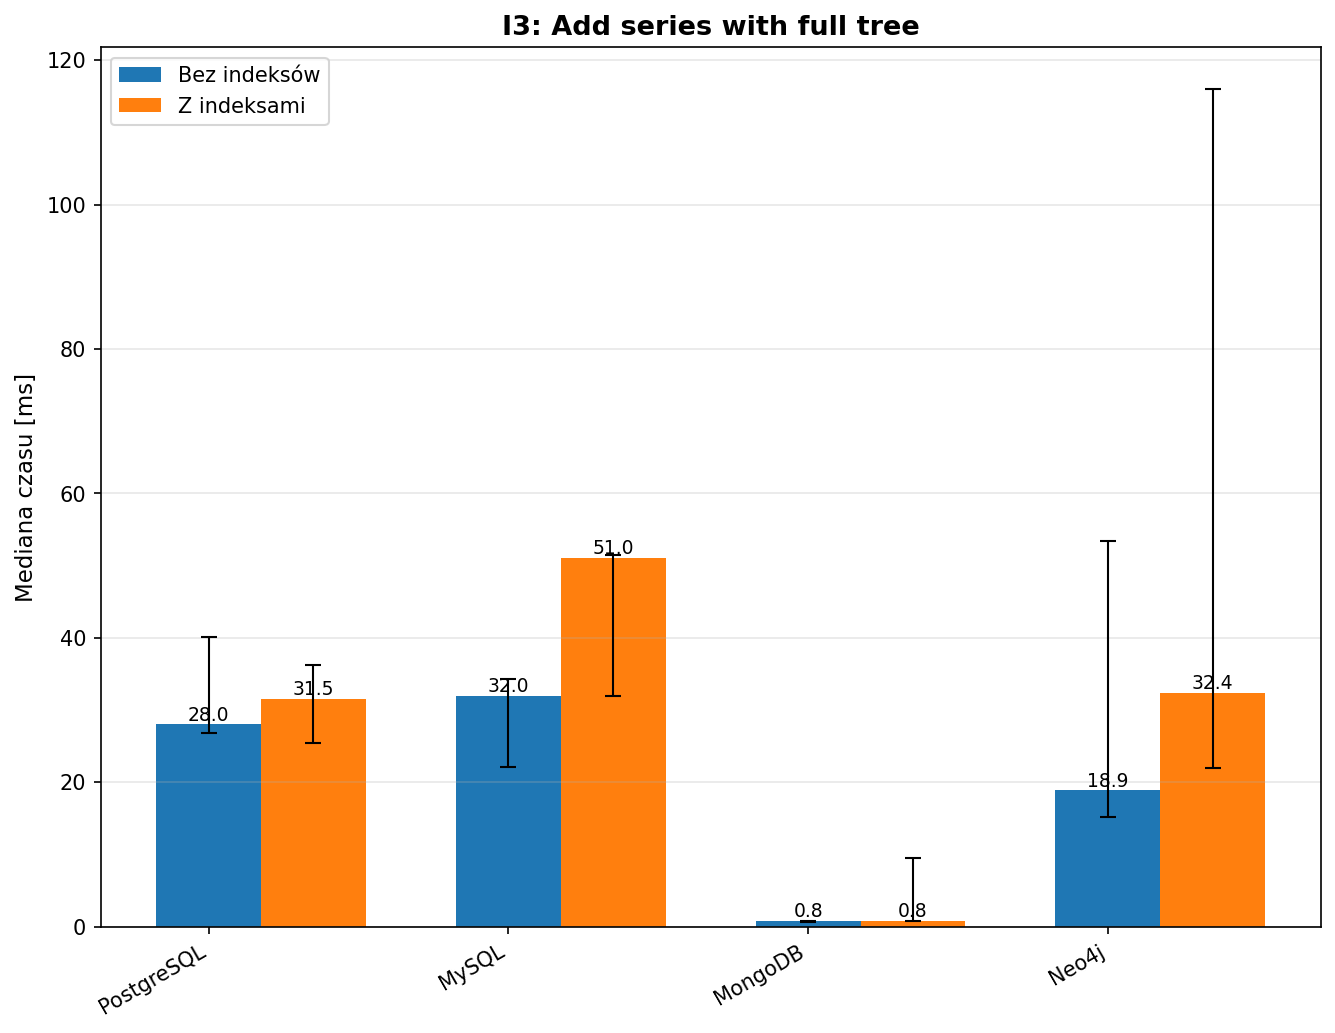
\includegraphics[width=0.8\textwidth]{charts/large/chart_I3.png}
    \caption{I3 -- Dodanie serialu z pełnym drzewem}
\end{figure}

Wynik praktycznie identyczny jak na \emph{small} i \emph{medium} --
MongoDB 0.8~ms, pozostali 18--51~ms. Niezależność od wolumenu
potwierdza się w pełni: koszt pojedynczego \texttt{INSERT}-a serialu
nie rośnie z rozmiarem katalogu, bo nowo wstawiany rekord zostaje
po prostu dopisany na końcu. Większy wolumen spowodował tylko
dwukrotny wzrost czasu w MySQL z indeksami (19 → 51~ms) -- to
narzut przebudowy indeksu \texttt{FULLTEXT} przy każdym dopisanym
rekordzie.

% -------------------------------------------------------
% SELECT
% -------------------------------------------------------

\subsubsection{S2: Filtrowanie kolaboratywne}
\begin{figure}[H]
    \centering
    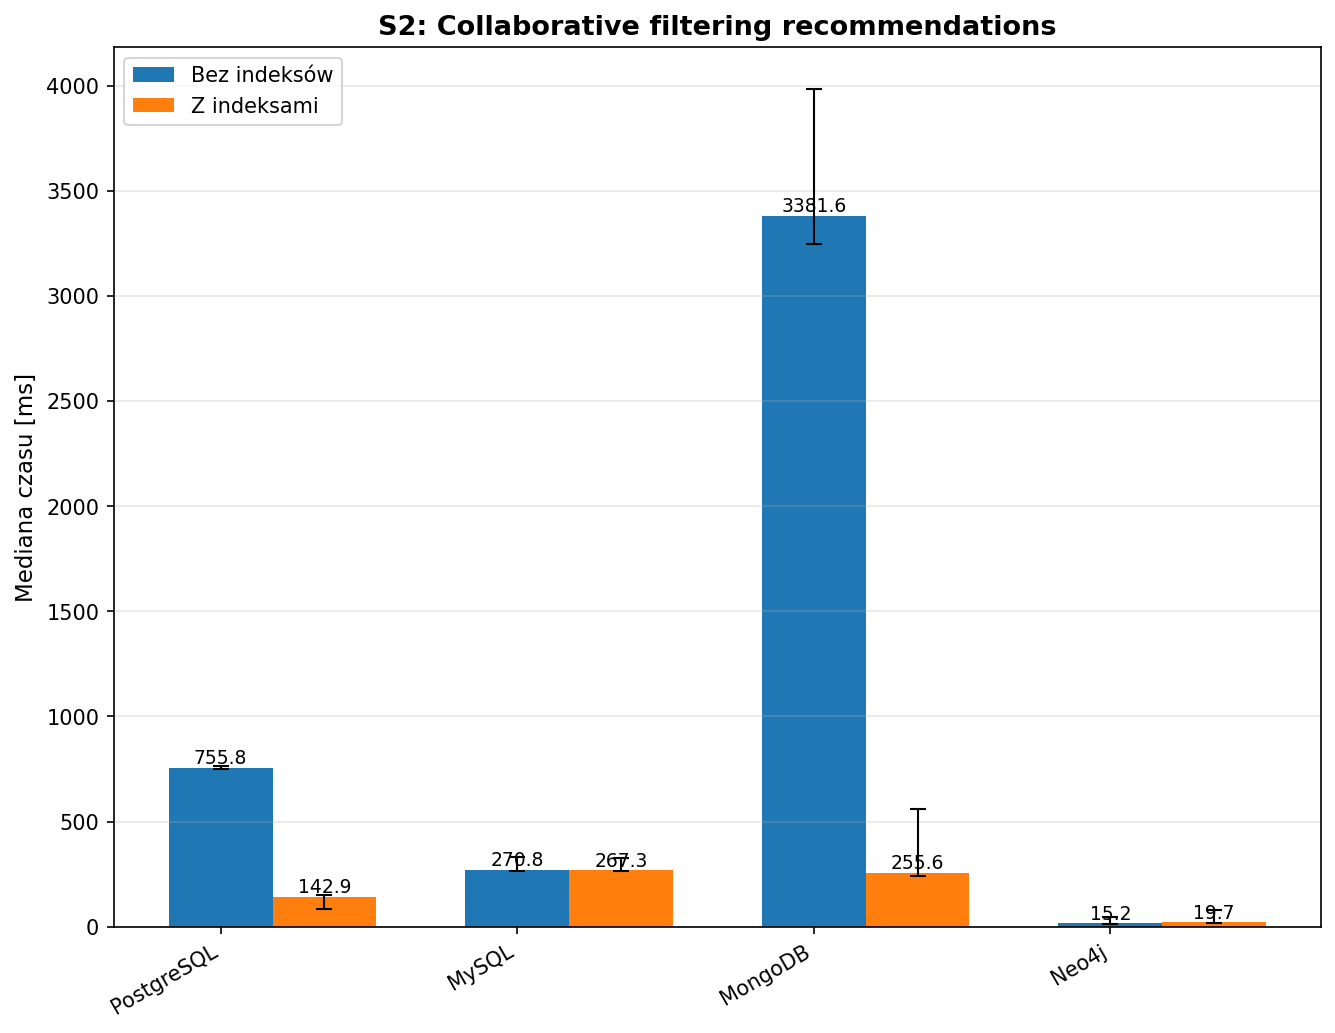
\includegraphics[width=0.8\textwidth]{charts/large/chart_S2.png}
    \caption{S2 -- Filtrowanie kolaboratywne}
\end{figure}

\textbf{Neo4j zostawia konkurencję daleko z tyłu} -- 15~ms bez
indeksów, 19~ms z indeksami. Pozostałe bazy bez indeksów osiągają sekundy:
PostgreSQL 755~ms, MySQL 270~ms, Mongo \emph{3.4~sekundy} (skan
6 milionów dokumentów). Z indeksami PG schodzi do 142~ms, Mongo do
255~ms -- ale Neo4j i tak pozostaje 8--15× szybszy. Ten scenariusz
najlepiej pokazuje, kiedy graf wygrywa: wielokrotne ,,wskakiwanie''
między profilami i treścią to nawigacja po krawędziach, w której
relacja jest fizycznym wskaźnikiem -- zamiast kolejnych \texttt{JOIN}-ów
po milionach wierszy.

\subsubsection{S3: TOP 100 według liczby ocen w okresie}
\begin{figure}[H]
    \centering
    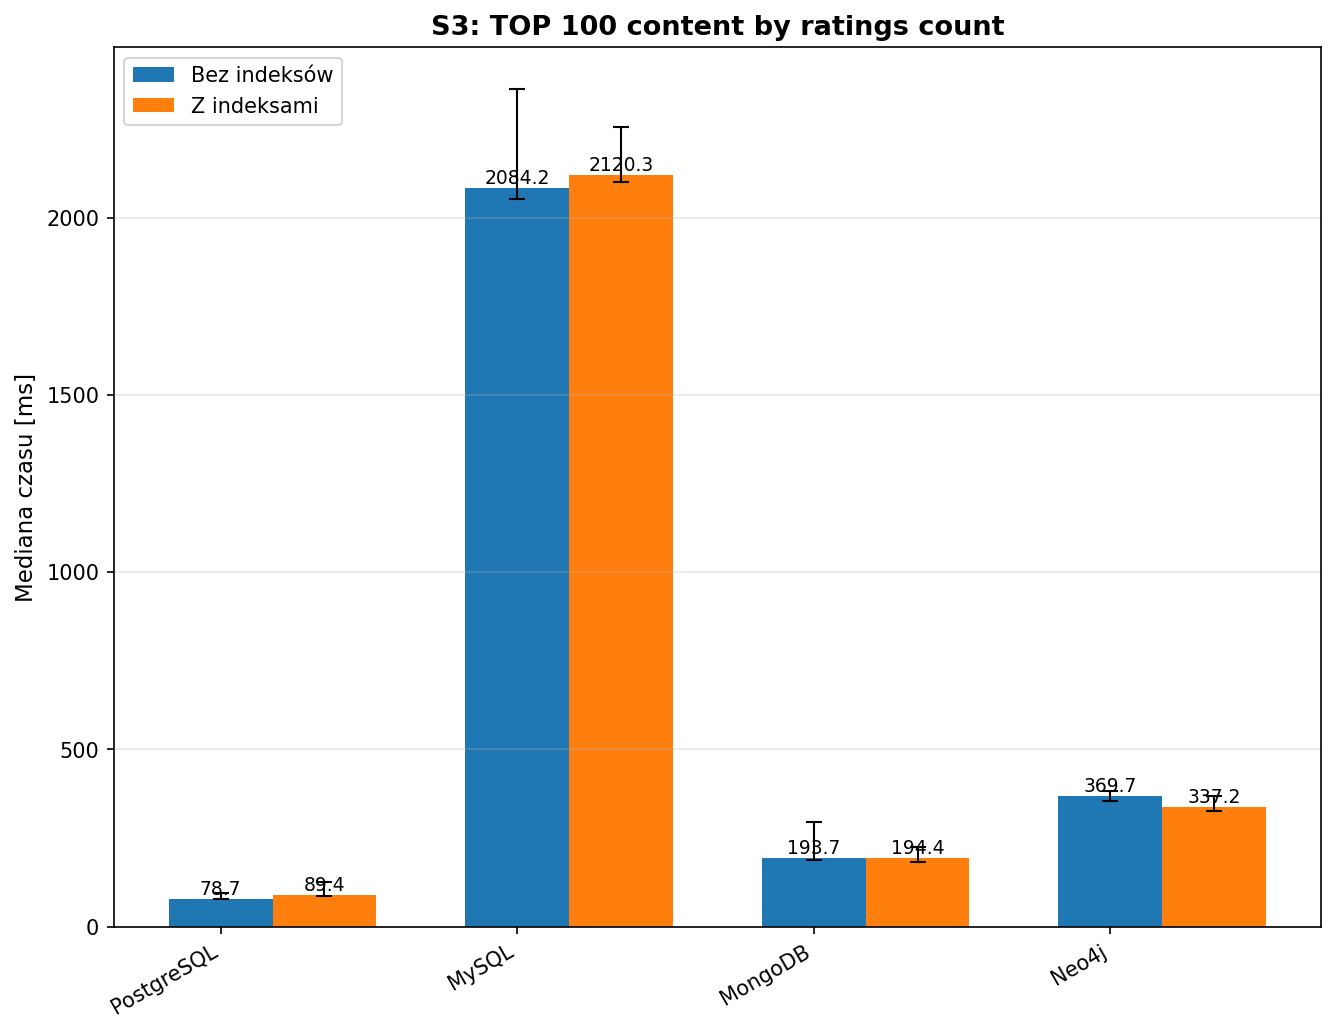
\includegraphics[width=0.8\textwidth]{charts/large/chart_S3.png}
    \caption{S3 -- TOP 100 według liczby ocen w okresie}
\end{figure}

Tu zaczynają się \emph{poważne} różnice. PostgreSQL nadal najszybszy
(79~ms), MySQL 2.1~sekundy(!), MongoDB 194~ms, Neo4j 370~ms. Indeksy
nie pomagają -- wszystkie warianty mają porównywalne czasy do
wariantu bez indeksów. PostgreSQL wygrywa dzięki efektywnemu
wykonaniu agregacji \texttt{COUNT(*)} z grupowaniem; MySQL traci
przez nieefektywny plan z pełnym skanem 5.7~mln wierszy
(potwierdzone w 11.3). To jeden z dwóch scenariuszy w pracy
(obok S2 dla Neo4j), w których architektura silnika znaczy
więcej niż obecność indeksu.

\subsubsection{S4: Wyszukiwanie pełnotekstowe po tytule}
\begin{figure}[H]
    \centering
    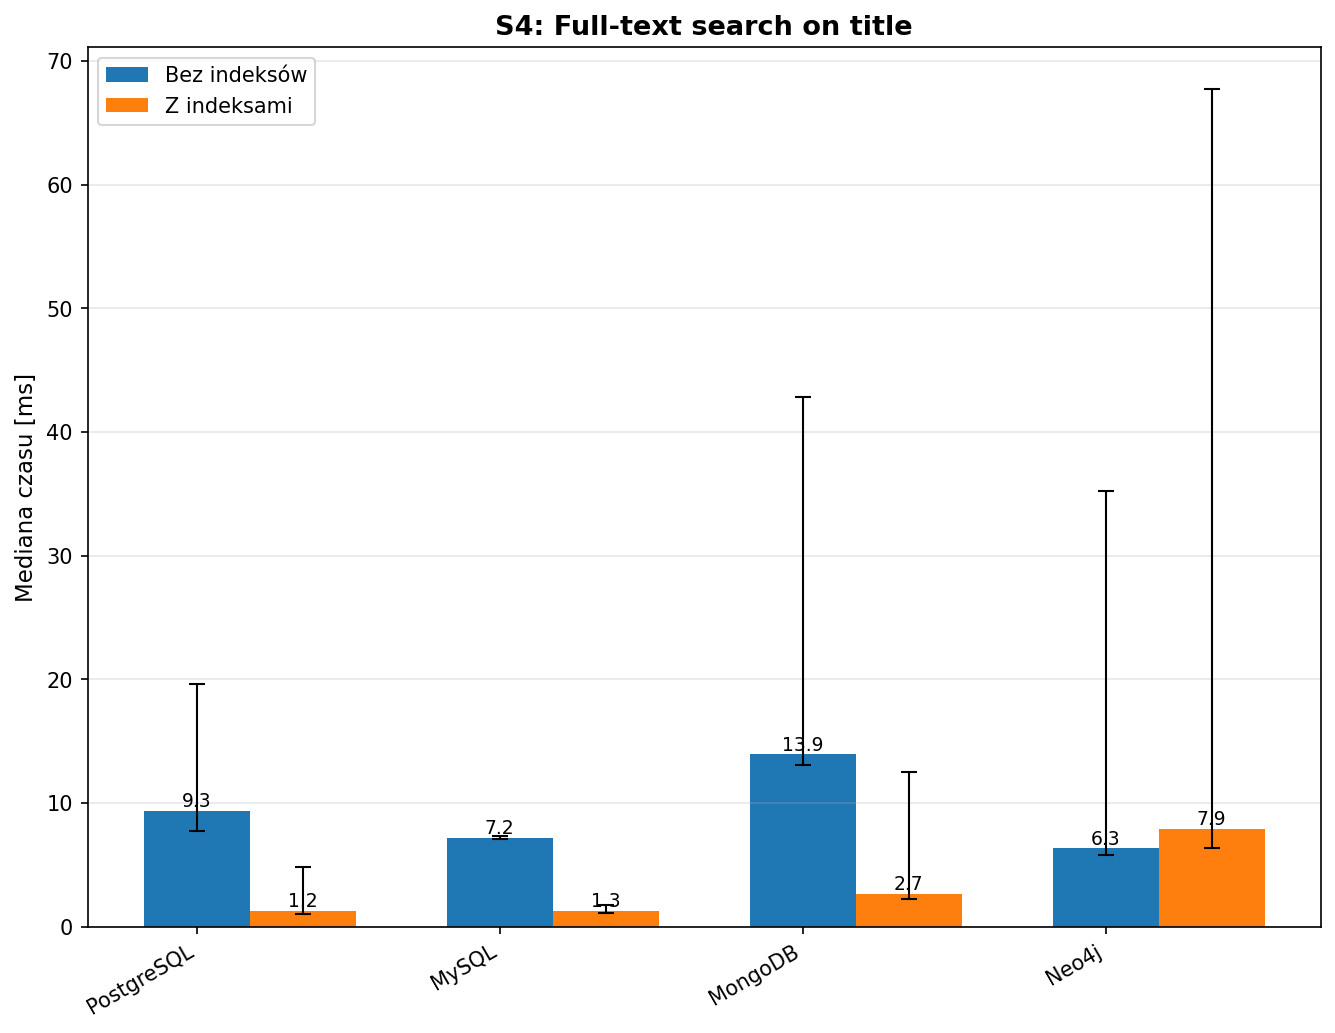
\includegraphics[width=0.8\textwidth]{charts/large/chart_S4.png}
    \caption{S4 -- Wyszukiwanie pełnotekstowe po tytule}
\end{figure}

Indeksy pełnotekstowe działają wzorowo -- bez nich silniki sięgają
7--14~ms (Neo4j najszybszy 6.3~ms dzięki temu, że i tak skanuje
,,tylko'' 15\,000 węzłów), z indeksami wszystkie spadają do
1--3~ms (poza Neo4j -- tam paradoksalnie wzrost do 7.9~ms,
możliwy artefakt cache'u Lucene). PostgreSQL z trygramowym GIN-em
schodzi do 1.2~ms -- ośmiokrotne przyspieszenie. MongoDB z indeksem
\texttt{text}: 2.7~ms (5×). To podręcznikowe potwierdzenie wartości
indeksu pełnotekstowego dla wyszukiwania po wzorcach z wiodącym
,,\%''.

% -------------------------------------------------------
% DELETE
% -------------------------------------------------------

\subsubsection{D1: Usunięcie treści z kaskadą}
\begin{figure}[H]
    \centering
    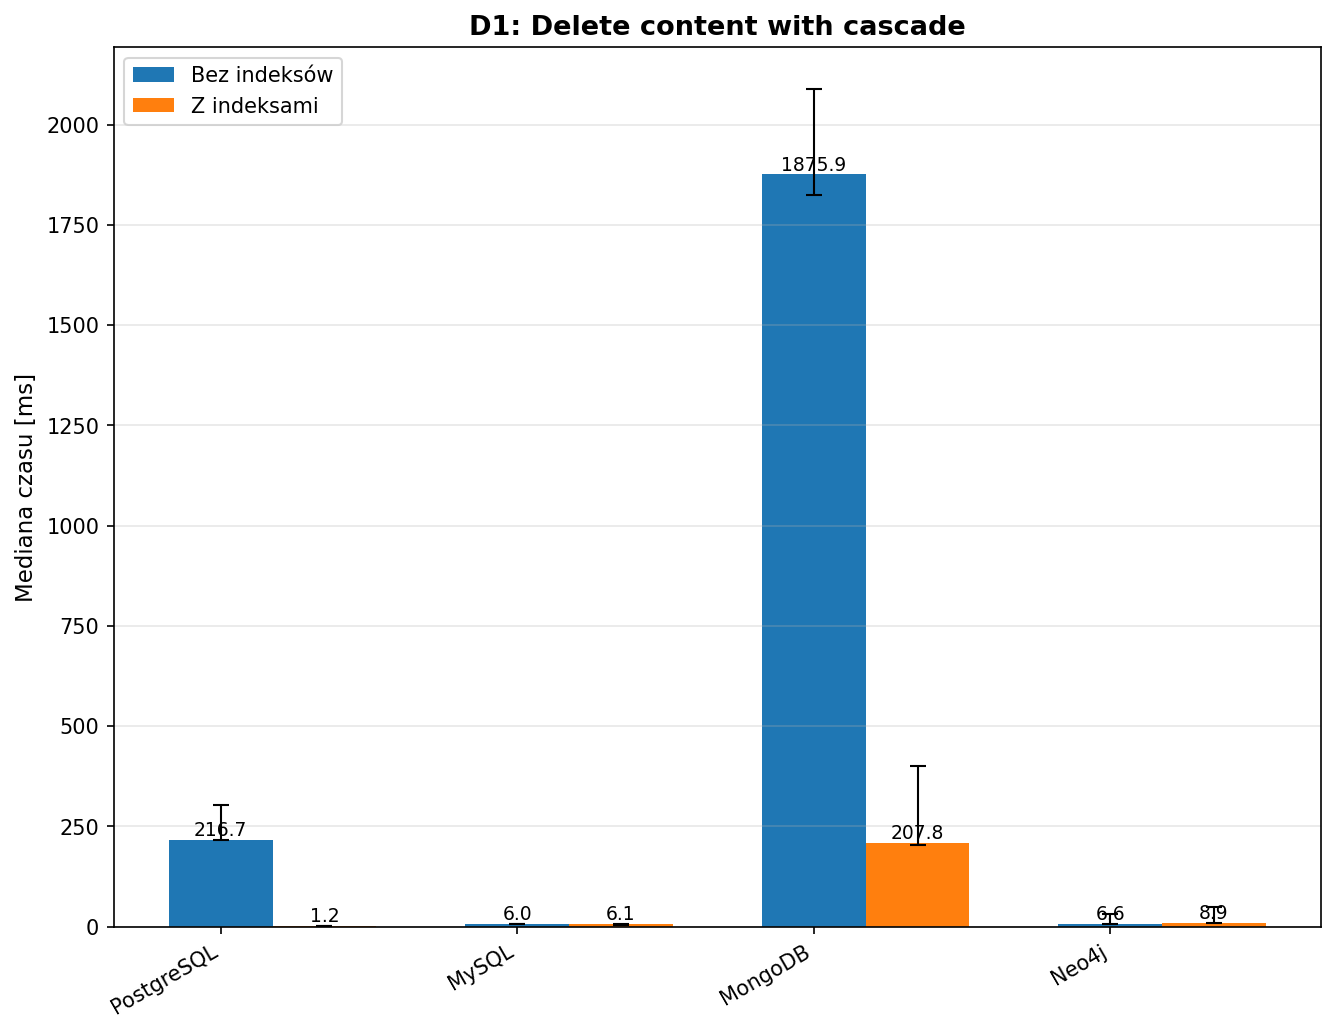
\includegraphics[width=0.8\textwidth]{charts/large/chart_D1.png}
    \caption{D1 -- Usunięcie treści z kaskadą}
\end{figure}

Skala potęguje efekt indeksu na FK. PostgreSQL bez indeksu --
\textbf{217~ms}, z indeksem \emph{1.2~ms} (180-krotne przyspieszenie).
MongoDB bez indeksu 1.9~sekundy(!), z indeksem 208~ms (9×).
Neo4j 7--9~ms niezależnie od wariantu -- relacje są wskaźnikami,
więc kaskada to natychmiastowe odnalezienie sąsiadów. MySQL stabilnie
6~ms (FK index nieusuwalny). Wniosek: dla tabel ze związkami
kaskadowymi indeks na kluczu obcym jest \emph{absolutną koniecznością}
-- bez niego każde usunięcie staje się skanem powiązanych tabel.

\subsubsection{D4: Usunięcie pozycji z listy}
\begin{figure}[H]
    \centering
    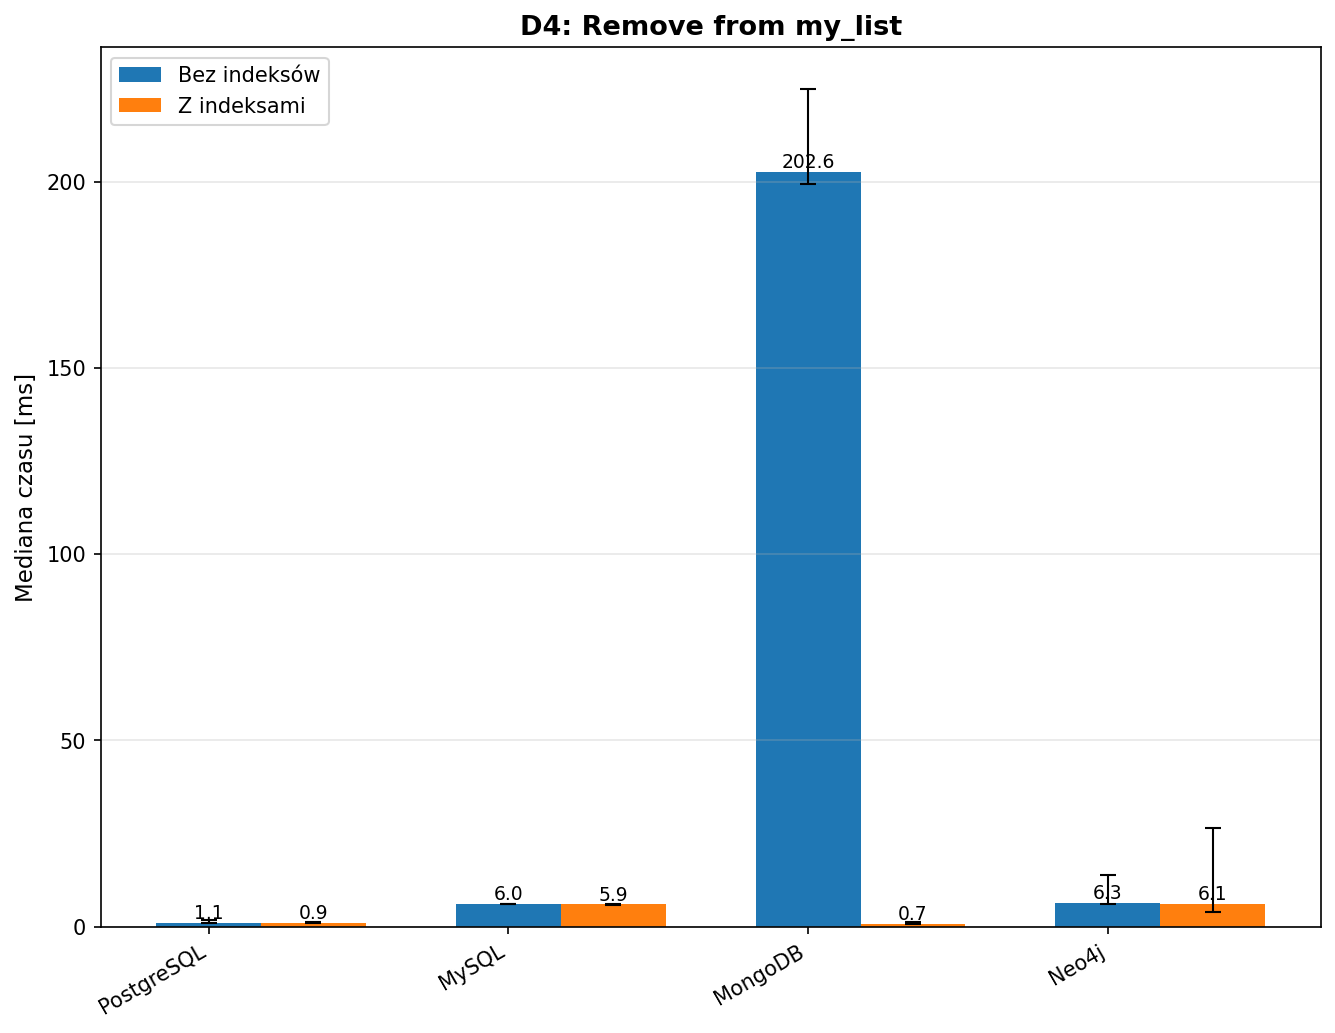
\includegraphics[width=0.8\textwidth]{charts/large/chart_D4.png}
    \caption{D4 -- Usunięcie pozycji z listy}
\end{figure}

MongoDB bez indeksu eskaluje do \textbf{202~ms} (z 20~ms na
\emph{small}) -- klasyczne liniowe skalowanie skanu kolekcji.
Z indeksem 0.7~ms -- \emph{286-krotna} różnica. To najsilniej
skalujący się dowód wartości indeksu w całej pracy. PostgreSQL
i Neo4j stałe poniżej 6~ms, MySQL stałe 6~ms. Operacja prosta,
ale dramatycznie różna w zachowaniu między modelem indeksowanym
a nieindeksowanym.

\subsubsection{D6: Masowe usunięcie nieaktywnych użytkowników}
\begin{figure}[H]
    \centering
    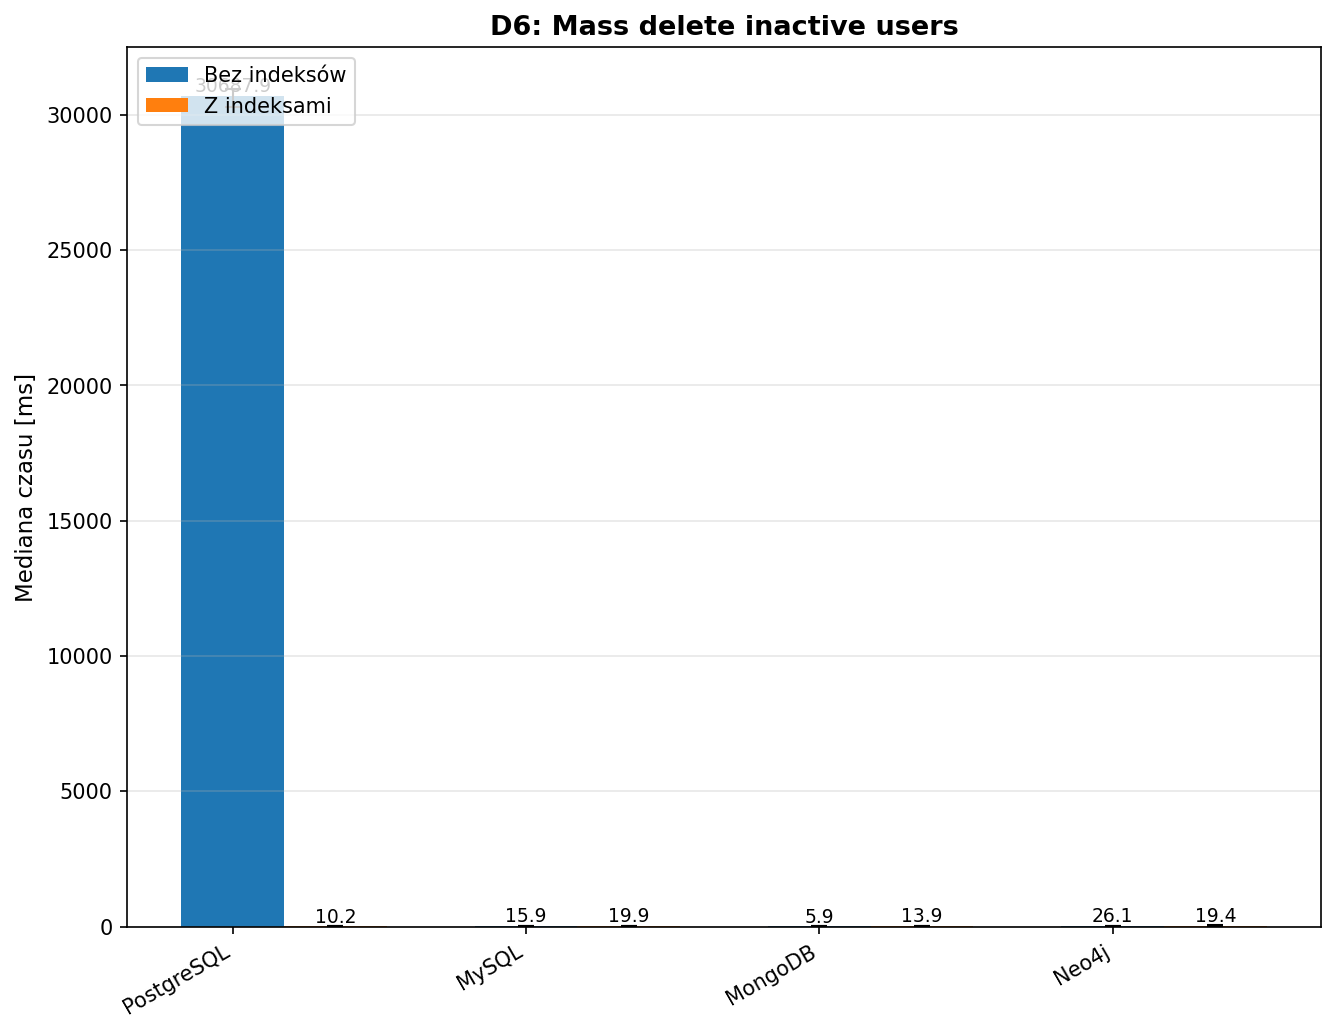
\includegraphics[width=0.8\textwidth]{charts/large/chart_D6.png}
    \caption{D6 -- Masowe usunięcie nieaktywnych użytkowników}
\end{figure}

Najbardziej spektakularny wynik całej pracy. PostgreSQL bez indeksu
na \texttt{users.status}: \textbf{30.7 sekundy}. Z indeksem:
\emph{10~milisekund}. To \textbf{3000-krotne} przyspieszenie --
indeks zmienia operację, która jest praktycznie niewykonalna
w produkcji w operację w czasie reakcji aplikacji webowej. MongoDB
i Neo4j również zyskują (5.9 → 13.9~ms i 26 → 19~ms odpowiednio),
ale bez tej dramatycznej skali. MySQL stabilnie 16--20~ms. Ten
scenariusz powinien być \emph{centralnym argumentem} pracy:
różnica trzy rzędów wielkości to nie kosmetyka, to różnica między
,,można uruchomić'' a ,,nie wolno wykonać''.

% -------------------------------------------------------
% UPDATE
% -------------------------------------------------------

\subsubsection{U2: Przeliczenie średniej oceny}
\begin{figure}[H]
    \centering
    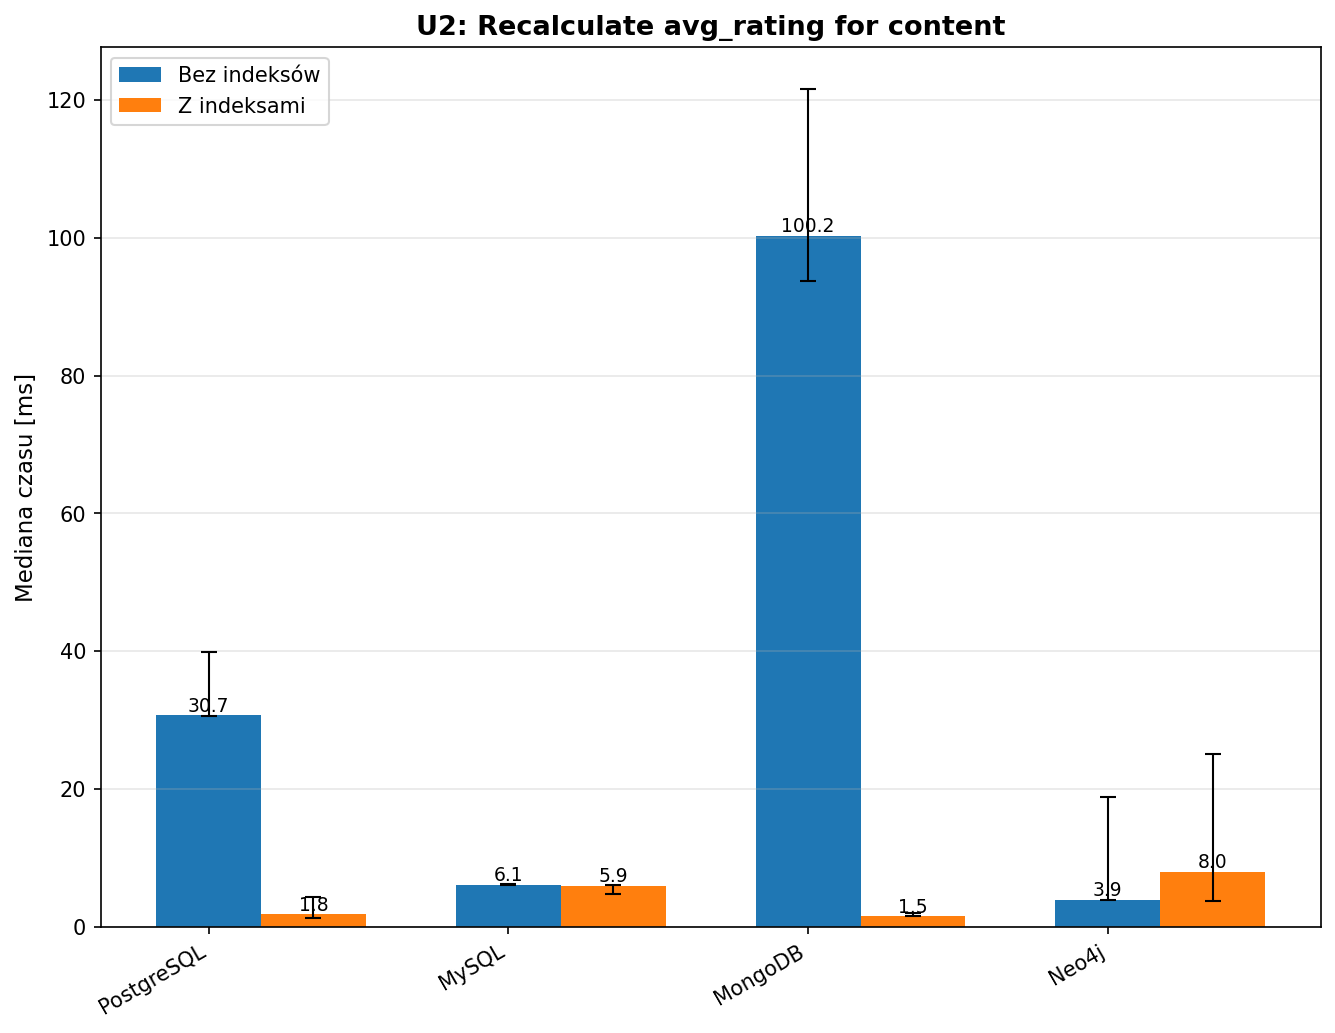
\includegraphics[width=0.8\textwidth]{charts/large/chart_U2.png}
    \caption{U2 -- Przeliczenie średniej oceny}
\end{figure}

Wzorzec ze \emph{small} i \emph{medium} się skaluje, ale kontrast
rośnie. PostgreSQL bez indeksu 30.7~ms (był 8.8~ms na \emph{medium}),
z indeksem 1.8~ms. MongoDB bez indeksu 100~ms, z indeksem 1.5~ms
(67×). MySQL i Neo4j stabilne 6 i 4--8~ms. Pojedynczy \texttt{UPDATE}
po agregacie -- kontrast między ,,znalezieniem wiersza'' z indeksem
a ,,znalezieniem wiersza'' przez skan jest tym wyraźniejszy, im więcej
wierszy do przeskanowania. Indeks działa idealnie zgodnie
z hipotezą.

\subsubsection{U3: Masowa zmiana planu subskrypcji}
\begin{figure}[H]
    \centering
    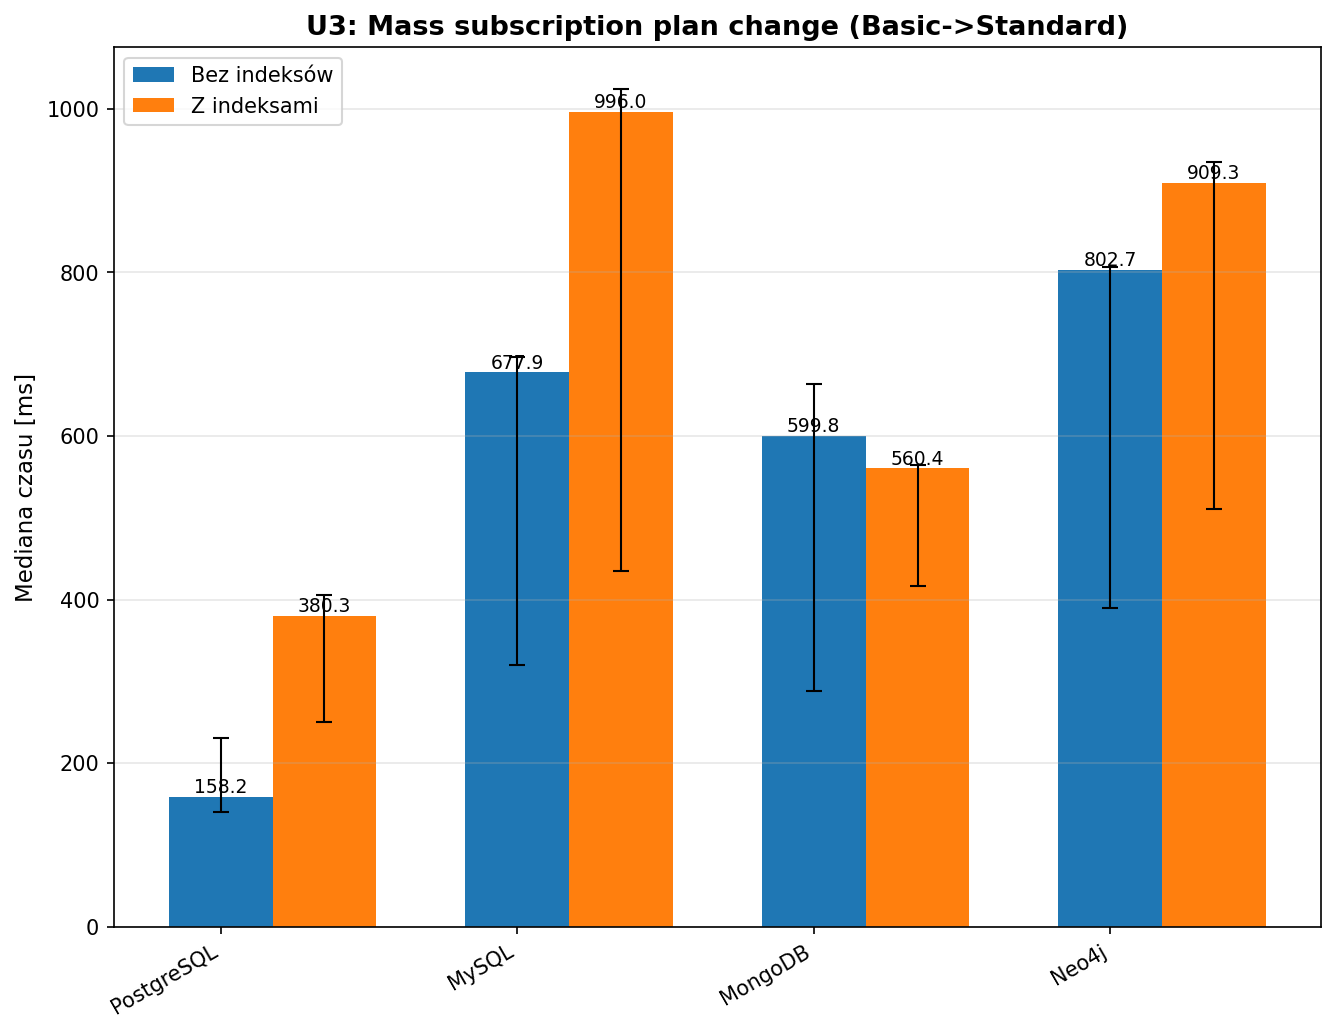
\includegraphics[width=0.8\textwidth]{charts/large/chart_U3.png}
    \caption{U3 -- Masowa zmiana planu subskrypcji}
\end{figure}

Koszt utrzymania indeksów przy modyfikacji wierszy osiąga tu
maksimum. PostgreSQL bez indeksu
158~ms, z indeksem \emph{380~ms} -- \textbf{2.4-krotne pogorszenie}.
MySQL 678 → 996~ms (1.5×), Neo4j 803 → 909~ms (1.1×), MongoDB
599 → 560~ms (lekko lepiej). Operacja modyfikuje pole \texttt{plan\_name}
na milionach wierszy -- każda zmiana wymusza przepisanie wpisu
w indeksie złożonym \texttt{(status, plan\_name)}. To jest
\emph{koronny dowód drugiej części hipotezy}: dla masowych
\texttt{UPDATE}-ów na kolumnach indeksowanych obecność indeksu
jest \emph{kosztem}, nie zyskiem. Razem z D6 ten scenariusz
domyka pełną diagnozę: indeks może być najlepszym przyjacielem
albo najgorszym wrogiem, w zależności od tego, czy operacja
\emph{czyta} czy \emph{pisze} po indeksowanej kolumnie.
